\lstset { %
    language=C++,
    backgroundcolor=\color{blue!10}, % set backgroundcolor
    basicstyle=\footnotesize,% basic font setting,
        commentstyle=\color[rgb]{0.026,0.112,0.095},
                basicstyle=\ttfamily,
                keywordstyle=\color{blue}\ttfamily,
                stringstyle=\color{red}\ttfamily,
                commentstyle=\color{gray}\ttfamily,
                morecomment=[l][\color{magenta}]{\#}
}
%--------------------------------------------------------------------------------------------------
%--------------------------------------------------------------------------------------------------
\begin{frame}

Part 0:
\vspace{0.2cm}

{\LARGE \textbf{\textcolor{blue}{Introduction}}}

\end{frame}
%--------------------------------------------------------------------------------------------------
%\begin{frame}[fragile]{\textcolor{blue}{Program}}
%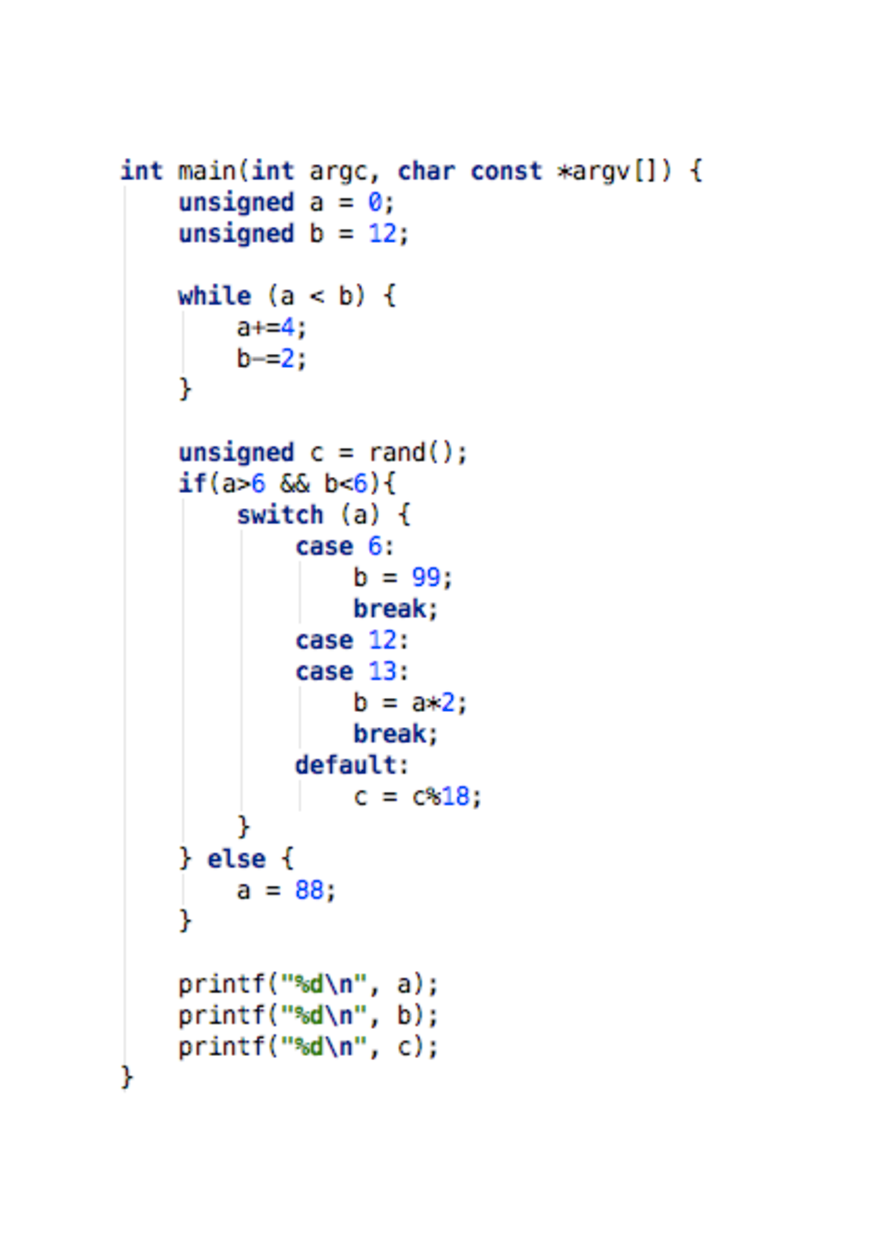
\includegraphics[scale=0.45]{src/example_c.pdf}
%\end{frame}
%--------------------------------------------------------------------------------------------------
\begin{frame}[fragile]{\textcolor{blue}{Motivation}}
%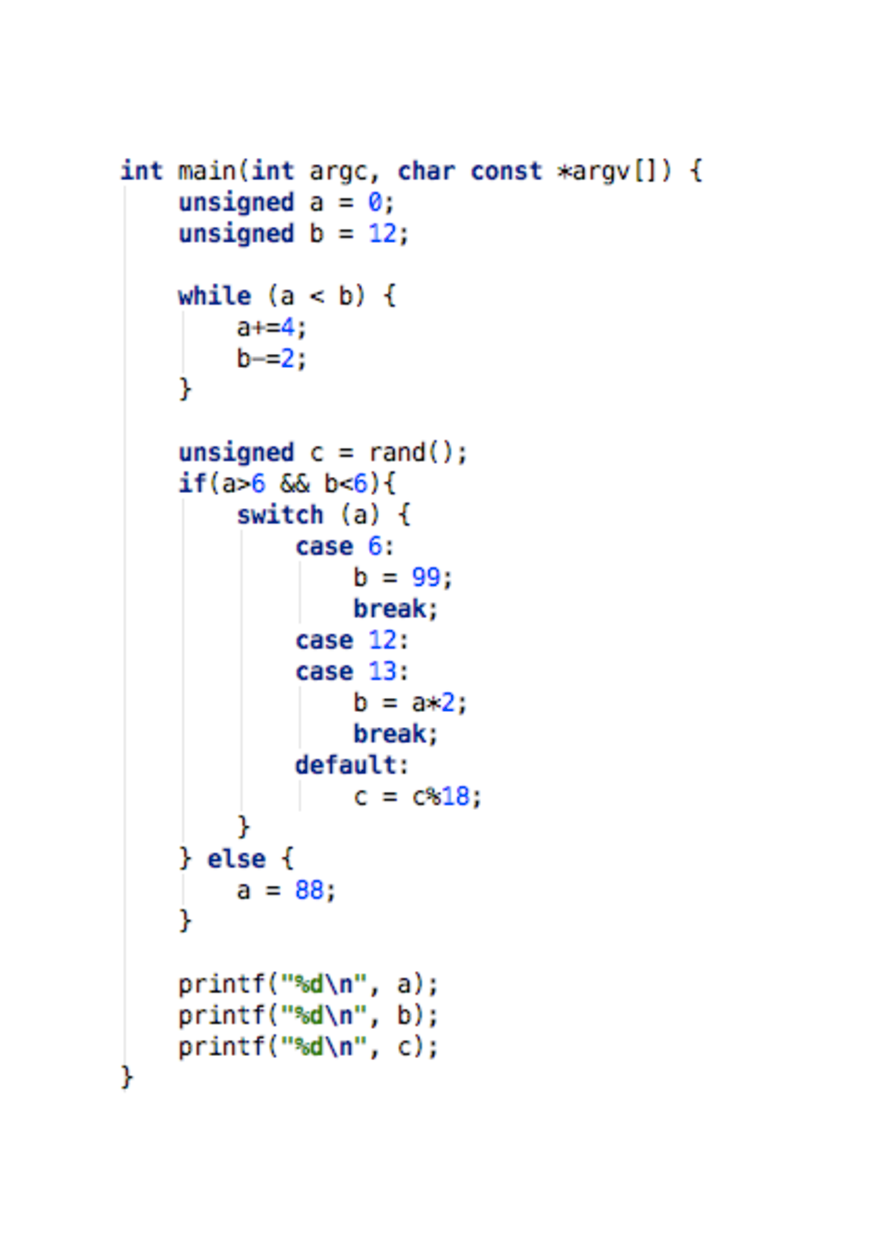
\includegraphics[scale=0.6]{src/example_c.pdf}
\begin{footnotesize}
\begin{lstlisting}[language=C++]
int main(int argc, char const *argv[]) {
    unsigned a = 0, b = 12, c = rand();

    while (a < b) { a+=4; b-=2; }

    if(a>6 && b<6){
        switch (a) {
            case  6: b = 99;  break;                 // reachable? 
            case 12:
            case 13: b = a*2; break;
            default:
                c = c%18;
        }
    } else {
        a = 88;
    }

    printf("%d\n", a);		// what will/might be printed out?
    printf("%d\n", b);
    printf("%d\n", c);
}
\end{lstlisting}
\end{footnotesize}
\end{frame}
%--------------------------------------------------------------------------------------------------
\begin{frame}[fragile]{\textcolor{blue}{Value Set Analysis}}

%\begin{minipage}{0.49\textwidth}

\underline{\smash{Bounded Set Analysis:}}
%\begin{itemize}
%\item
\begin{align*}
Var \,\rightarrow\,\{a,\,b,\,c,\,...\}_n
\end{align*}
%\end{itemize}

\underline{\smash{Interval Analysis:}}
%\begin{itemize}
%\item
\begin{align*}
Var \,\rightarrow\, [a:b]_n
\end{align*}
%\end{itemize}

\underline{\smash{Strided Interval Analysis:}}
%\begin{itemize}
%\item
\begin{align*}
Var \,\rightarrow\,s[a:b]_n
\end{align*}
%\end{itemize}
%\end{minipage}

\vspace{1.0cm}

SSA: sufficient to store the {\color{blue}abstract value for each variable once per basic block}:\footnote{The need to store it not just once only arises to preserve information at conditional branches.}
\begin{align*}
\mathcal{D}\,:\, BB \,\rightarrow\, Var \, \rightarrow\, Val
\end{align*}

\end{frame}
%--------------------------------------------------------------------------------------------------

\begin{frame}[fragile]{\textcolor{blue}{Passes in LLVM}}
LLVM's analysis and optimization framework {\color{blue} opt}:

\begin{center}
C/C++ 
\tikzfancyarrow{Clang} 
IR
\tikzfancyarrow{opt}
IR
\tikzfancyarrow{codegen}
machine code
\end{center}

\vspace{-0.3cm}

\hspace{4.4cm}
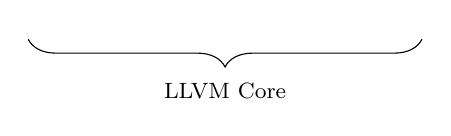
\begin{tikzpicture}[scale=1]
%\draw[thick] (-1,0) rectangle +(6,7.5);
\draw [decorate,decoration={brace,amplitude=10pt,mirror,raise=4pt},yshift=0pt]
(3.5,0.0) -- (8.5,0.0) node [black,midway,yshift=-0.8cm] {\footnotesize
LLVM Core};
\end{tikzpicture}

\vspace{0.9cm}

using existing passes (from command line):
\begin{footnotesize}
\begin{lstlisting}[language=C++]
opt -load -mem2reg -o hello-opt.bc < hello.bc
\end{lstlisting}
\end{footnotesize}
running user passes:
\begin{footnotesize}
\begin{lstlisting}[language=C++]
opt -load llvm/lib/llvm-vsa.so -vsapass -o hello.bc < hello.bc
\end{lstlisting}
\end{footnotesize}

\end{frame}
%--------------------------------------------------------------------------------------------------
\begin{frame}[fragile]{\textcolor{blue}{Passes in LLVM (cont.)}}
\underline{\smash{Creating user passes:}}
\begin{itemize}
\item inherit from existing passes (module, function, block):
\begin{footnotesize}
\begin{lstlisting}[language=C++]
struct ThisPass : public ModulePass {}
\end{lstlisting}
\end{footnotesize}

\item specify required passes, which have to be run in advance:
\begin{footnotesize}
\begin{lstlisting}[language=C++]
void ThisPass::getAnalysisUsage(AnalysisUsage &AU) override {
  AU.setPreservesAll();
  AU.addRequired<OtherPass>();
}
\end{lstlisting}
\end{footnotesize}

\item perform analysis by using/accessing results of other passes:
\begin{footnotesize}
\begin{lstlisting}[language=C++]
bool ThisPass::runOnModule(Module &M) override {
  auto& other_result =  
    getAnalysis<OtherPass>(function).getResult();
  /* ... perform analysis and fill result ... */
  
  // Return if the pass modified the bitcode (no)
  return false;
}
\end{lstlisting}
\end{footnotesize}

\item make results available for other pass (optional): 
\begin{footnotesize}
\begin{lstlisting}[language=C++]  
ThisResult& ThisPass::getResult(){ return result; }
\end{lstlisting}
\end{footnotesize}

\end{itemize}

\end{frame}
%--------------------------------------------------------------------------------------------------
\begin{frame}[fragile]{\textcolor{blue}{LLVM's Intermediate Representation IR}}
\begin{center}
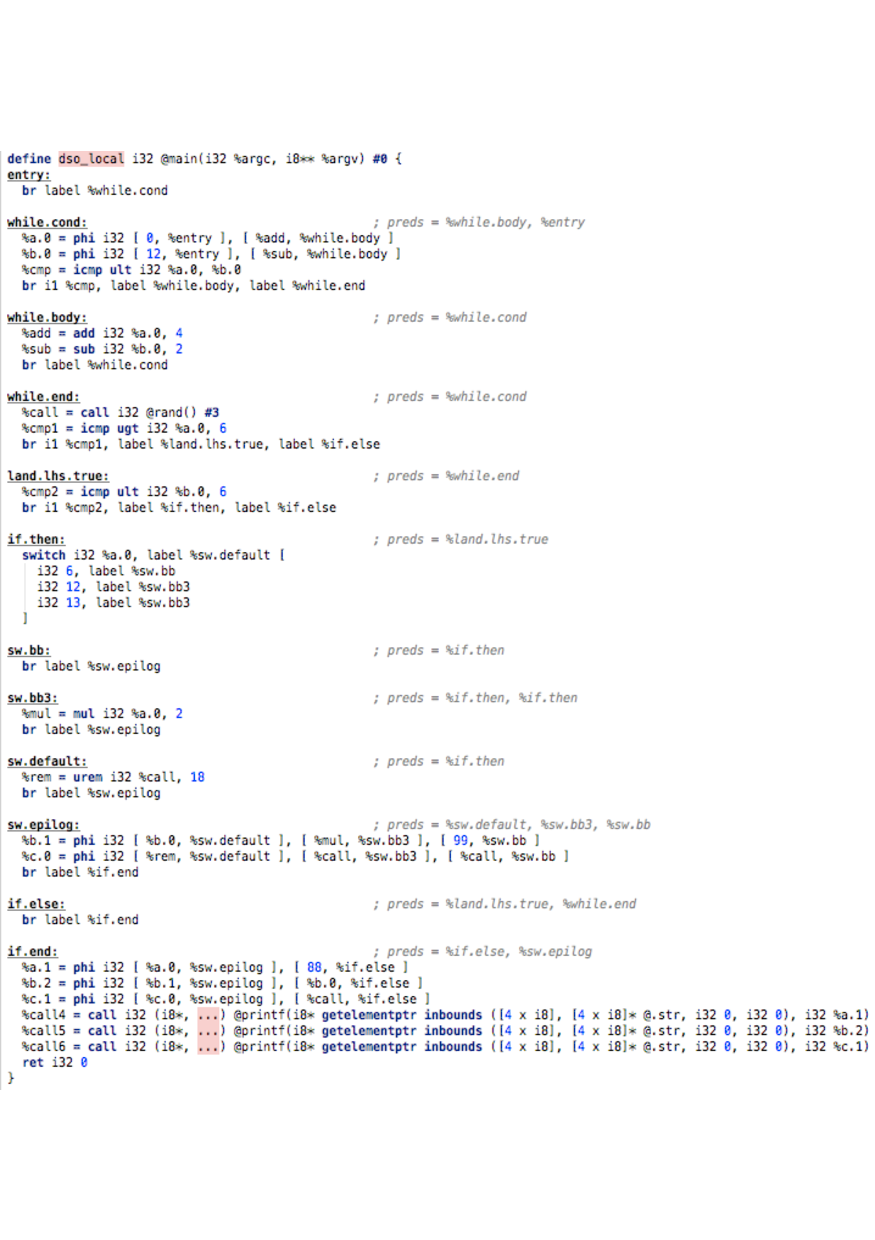
\includegraphics[width=0.7\textwidth, trim={0.1cm 12cm 4.5cm 2.5cm},clip]{src/example_ll.pdf} 
\end{center}

\hfill ... and many more lines of code
\end{frame}
%--------------------------------------------------------------------------------------------------
\begin{frame}[fragile]{\textcolor{blue}{Content of the Lab}}

\underline{Tasks:}
\begin{itemize}
\item implement {\color{blue}abstract domain}s that suitably represent value sets
\item develop a new analysis tool in LLVM to determine the value set of each \\
\qquad variable, using visitor and fixpoint algorithm (worklist) $\triangleright$ {\color{blue} VSAPass}
\item make results accessible via API: {\color{blue} VSAResult} and {\color{blue} VSAResultValue}
\item compare results with LLVM's {\color{blue} LazyValueInfo}
\end{itemize}

\vspace{1cm}

\underline{\smash{Future work:}}
\begin{itemize}
\item widening and narrowing
\item inter-procedural analysis
\item memory access 
\end{itemize}
\hfill unknowns (ops, return values and arguments of functions) treated as: {\color{blue} $\top$}

\end{frame}
%--------------------------------------------------------------------------------------------------